\documentclass[border=10pt]{standalone}
\usepackage{tikz}
\usetikzlibrary{arrows.meta, positioning, shadows}

\definecolor{boxblue}{HTML}{e8f4f8}
\definecolor{boxborder}{HTML}{2c3e50}

\tikzset{
    model/.style={
        rectangle, rounded corners=4pt,
        draw=boxborder, fill=boxblue,
        minimum width=4.2cm, minimum height=1.2cm,
        text width=4cm, align=center,
        font=\small, drop shadow={shadow xshift=0.5mm, shadow yshift=-0.5mm}
    },
    edge label/.style={
        font=\scriptsize\itshape, text=boxborder, fill=white,
        inner sep=2pt, rounded corners=1pt
    },
    arr/.style={
        -Stealth, thick, color=boxborder
    }
}

\begin{document}
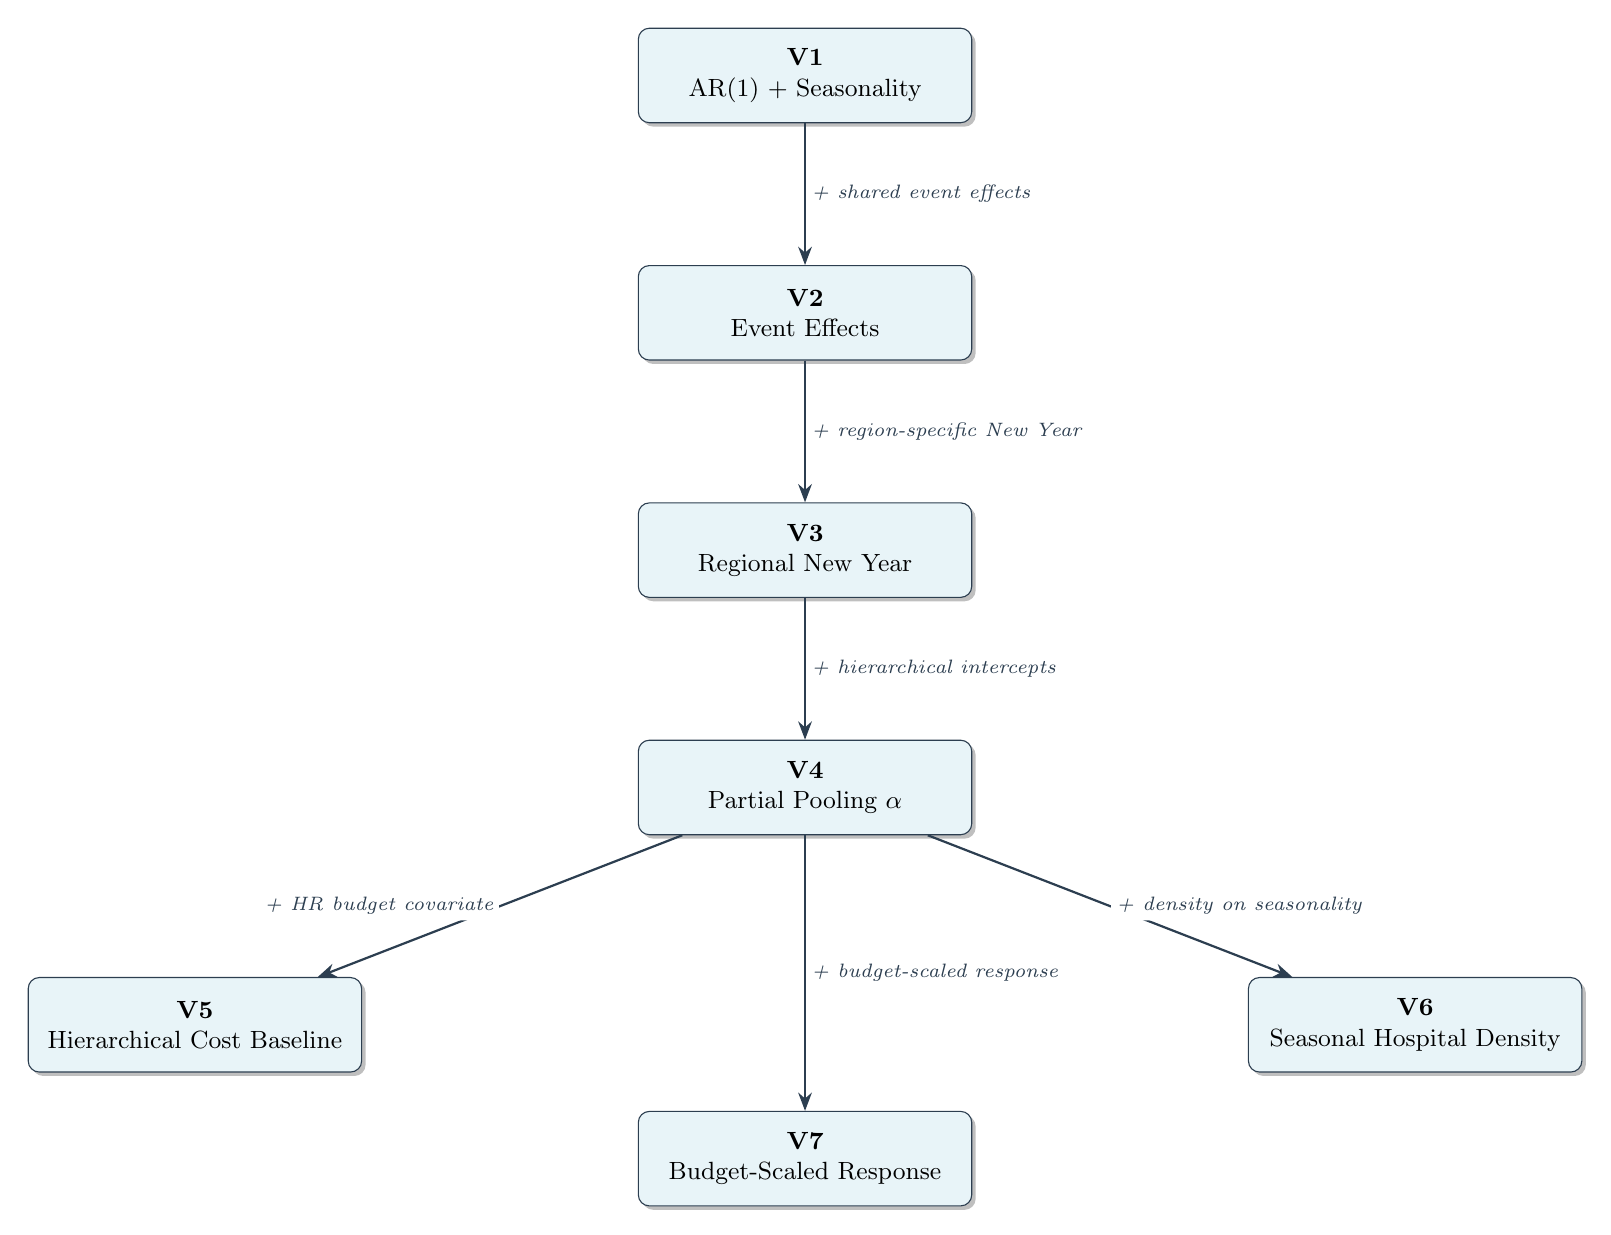
\begin{tikzpicture}[node distance=1.8cm and 3.5cm]

    % Nodes
    \node[model] (v1) {\textbf{V1}\\AR(1) + Seasonality};
    \node[model, below=of v1] (v2) {\textbf{V2}\\Event Effects};
    \node[model, below=of v2] (v3) {\textbf{V3}\\Regional New Year};
    \node[model, below=of v3] (v4) {\textbf{V4}\\Partial Pooling $\alpha$};
    \node[model, below left=of v4] (v5) {\textbf{V5}\\Hierarchical Cost Baseline};
    \node[model, below right=of v4] (v6) {\textbf{V6}\\Seasonal Hospital Density};
    \node[model, below=3.5cm of v4] (v7) {\textbf{V7}\\Budget-Scaled Response};

    % Edges
    \draw[arr] (v1) -- node[edge label, right] {+ shared event effects} (v2);
    \draw[arr] (v2) -- node[edge label, right] {+ region-specific New Year} (v3);
    \draw[arr] (v3) -- node[edge label, right] {+ hierarchical intercepts} (v4);
    \draw[arr] (v4) -- node[edge label, left] {+ HR budget covariate} (v5);
    \draw[arr] (v4) -- node[edge label, right] {+ density on seasonality} (v6);
    \draw[arr] (v4) -- node[edge label, right] {+ budget-scaled response} (v7);

\end{tikzpicture}
\end{document}
